%\documentclass[mathserif]{beamer}
\documentclass[handout]{beamer}
%\usetheme{Goettingen}
%\usetheme{Warsaw}
\usetheme{Singapore}



%\usetheme{Frankfurt}
%\usetheme{Copenhagen}
%\usetheme{Szeged}
%\usetheme{Montpellier}
%\usetheme{CambridgeUS}
%\usecolortheme{}
%\setbeamercovered{transparent}
\usepackage[english, activeacute]{babel}
\usepackage[utf8]{inputenc}
\usepackage{amsmath, amssymb}
\usepackage{dsfont}
\usepackage{graphics}
\usepackage{cases}
\usepackage{graphicx}
\usepackage{pgf}
\usepackage{epsfig}
\usepackage{amssymb}
\usepackage{multirow}	
\usepackage{amstext}
\usepackage{algorithm2e}
\usepackage{amsmath}
\usepackage{epic}
\usepackage{epsfig}
\usepackage{fontenc}
\usepackage{framed,color}
\usepackage{palatino, url, multicol}
%\algsetup{indent=2em}
\newcommand{\factorial}{\ensuremath{\mbox{\sc Factorial}}}
\newcommand{\BIGOP}[1]{\mathop{\mathchoice%
{\raise-0.22em\hbox{\huge $#1$}}%
{\raise-0.05em\hbox{\Large $#1$}}{\hbox{\large $#1$}}{#1}}}
\newcommand{\bigtimes}{\BIGOP{\times}}
 \vspace{-0.5cm}
\title{Annotate-Sample-Average (ASA): A New Distant Supervision Approach for Twitter Sentiment Analysis}
\vspace{2cm}
\subtitle[ECAI'16]{22nd European Conference on Artificial Intelligence\\ The Hague, The Netherlands}
  
\author[Felipe Bravo Márquez]{\footnotesize
%\author{\footnotesize  
Felipe Bravo-Marquez, Eibe Frank, and Bernhard Pfahringer} 
    
 
%\vspace{-0.3cm}
\institute{University of Waikato \\ Computer Science Department }

\titlegraphic{\includegraphics[scale=0.3]{../../img/waikato.png}}



\date{31 August, 2016}

\begin{document}
\begin{frame}
\titlepage


\end{frame}


\begin{frame}{Social Media}
\begin{scriptsize}
\begin{itemize}
 \item Microblogging services are increasingly being adopted by people in order to access and publish information.  
 \item \textbf{Twitter}: Massively used Microblogging platform where users post messages (a.k.a \textbf{tweets}) limited to 140 characters. 
 \item Tweets use a unique \textbf{informal dialect} including many abbreviations, acronyms, misspelled words, hashtags, and emoticons, e.g., \textbf{lol}, \textbf{omg}, \textbf{hahaha}, \textbf{\#hatemonday}, \textbf{:)} .
\end{itemize}
  \begin{figure}[h]
        	
\includegraphics[scale = 0.2]{pics/twitter.png}
        \end{figure}

\end{scriptsize}
\end{frame}



\begin{frame}{Sentiment Analysis and Social Media}
\begin{scriptsize}
\begin{itemize}
 \item  Twitter users tend to publish \textbf{personal opinions} regarding certain topics and news events. 
 
 \begin{enumerate}
  \footnotesize{
  \item Hey @Apple, pretty much all your products are amazing.  You blow minds every time you launch a new gizmo. That said, your hold music is crap.
 \item \#windows sucks...  I want \#imac so bad!!!  why is it so damn expensive :( @apple please give me free imac and I will love you :D}
 \end{enumerate}

 
 \item Analysing the sentiment underlying these opinions has important applications in product \textbf{marketing} and \textbf{politics}.
 
   \begin{figure}[h]
        	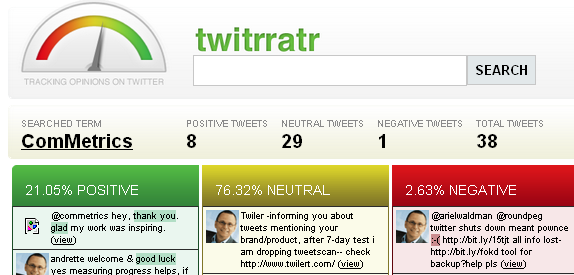
\includegraphics[scale = 0.4]{pics/tweetOpinions.png}
        \end{figure}
\end{itemize}
\end{scriptsize}

\end{frame}


\begin{frame}{Opinion Mining or Sentiment Analysis}
\begin{scriptsize}\begin{itemize}
 \item Application of \textbf{NLP} and \textbf{text mining} techniques to identify and extract subjective information from textual datasets.
\end{itemize}

\begin{block}{Message-level Polarity Classification (MPC) of Tweets}
  \begin{itemize}
   \item Automatically classify a tweet to classes \textcolor[rgb]{0.00,0.00,1.00}{\textbf{positive}}, \textcolor[rgb]{1.00,0.00,0.00}{\textbf{negative}}, or \textcolor[rgb]{0.00,1.00,0.00}{\textbf{neutral}}. 
   
     \begin{figure}[h]
        	
\includegraphics[scale = 0.15]{pics/sent.png}
        \end{figure}
   
   \item State-of-the-art solutions use \textbf{supervised} machine learning models trained from \textbf{manually} annotated examples \cite{NRCJAIR14}.
  \item \textbf{The Label Sparsity Problem}: manual annotation is \textbf{labour-intensive} and \textbf{time-consuming}. 
  \end{itemize} 
\end{block}

\end{scriptsize}

\end{frame}


\begin{frame}{Distant Supervision}
\begin{scriptsize}
  \begin{itemize}
  \item The label sparsity problem can be addressed using \textbf{Distant Supervision}.
   \item Automatically \textbf{label} unlabelled data (\textbf{Twitter API}) using a heuristic method~\cite{Mintz2009}.
     \item Unlabelled tweets are \textbf{cheap} to optain :)
   \item \textbf{Emoticon-Annotation Approach (EAA)}: tweets with positive \textcolor[rgb]{0.00,0.00,1.00}{\textbf{:)}} or negative \textcolor[rgb]{1.00,0.00,0.00}{\textbf{:(}} emoticons are labelled according to the polarity indicated by the emoticon~\cite{Read2005}.
  \item The emoticon is \textbf{removed} from the content.
\item Drawback: emoticons are \textbf{rarely} used in certain domains such as politics. 
    \end{itemize} 

   

\end{scriptsize}

\end{frame}







\begin{frame}{Lexicon-based Distant Supervision}
\begin{scriptsize}
\begin{itemize}
 \item We propose a  distant supervision method that builds \textbf{synthetically labelled tweets} based on \textbf{opinion lexicons} (we go beyond emoticons).
 
 \item  An opinion lexicon $\mathcal{L}$ is a lists of terms labelled by sentiment.
\item They are normally composed of positive and negative words such as \textcolor[rgb]{0.00,0.00,1.00}{\textbf{happy, wonderful}} and \textcolor[rgb]{1.00,0.00,0.00}{\textbf{sad, bad}}.


 \item Proposed method generate positive and negative training instances by \textbf{averaging} tweets containing words with the \textbf{same} polarity.
 
 \item Tweets are represented by \textbf{sparse feature vectors}.

 
\end{itemize}
\end{scriptsize}

\end{frame}



\begin{frame}{Lexical Polarity Hypothesis}
\begin{scriptsize}
\begin{itemize}

\item A tweet containing a word with a certain polarity is more likely to express the \textbf{same polarity} than the \textbf{opposite} $p_d>0.5$ (Bernoulli experiment).



 \begin{figure}[htb]
\begin{center}
\scalebox{0.3}{
\begin{tabular}{cc}
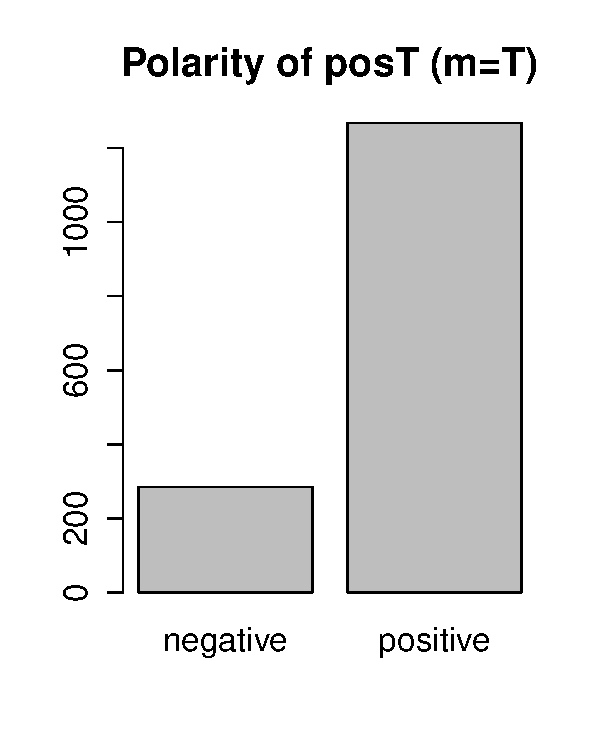
\includegraphics{pics/posTmT.pdf} &  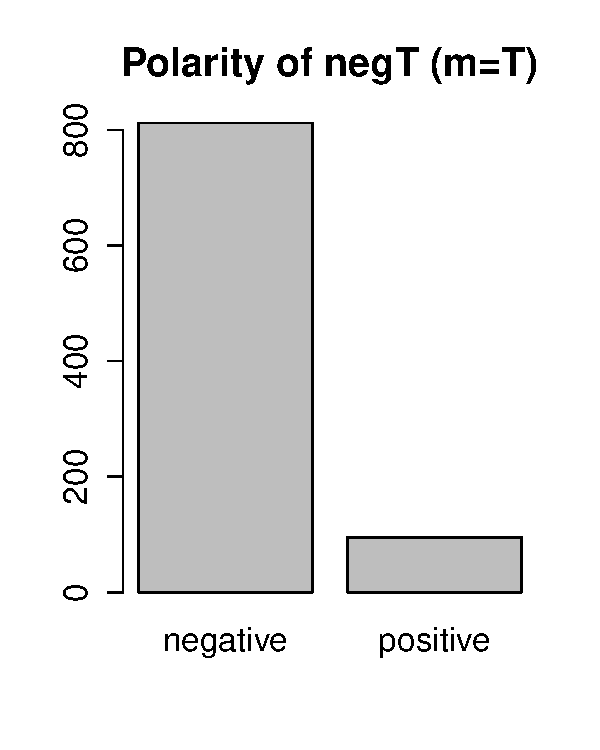
\includegraphics{pics/negTmT.pdf}  \\
\end{tabular}}
\label{fig:barplots}
\end{center}
\end{figure}

\item The opposite polarity may also be expressed due to the presence of  \textbf{negation}, \textbf{sarcasm}, or other opinion words with the \textbf{opposite} polarity.

\end{itemize}
\end{scriptsize}

\end{frame}


\begin{frame}{Why Averaging?}
\begin{scriptsize}
\begin{itemize}
\item Averaging multiple tweets with words with the same polarity \textbf{increases} the confidence of generating instances located in the \textbf{region} of the desired polarity.
\item We assume that the average tweet will behave similarly to the \textbf{majority}.
\item Probability that the \textbf{majority} of the tweets sampled from a collection of tweets with at least one word with the target polarity have the desired polarity:
\begin{displaymath}
 P(M) = \sum_{i=\lfloor \frac{a}{2}\rfloor +1}^a \binom a i  p_d^i(1-p_d)^{a-i}
\end{displaymath}
         
\begin{table}
\begin{center}
\scalebox{0.7}{
\begin{tabular}{|l|l|l|l|l|}
\hline
 & $p_d = 0.6$ & $p_d = 0.7$ & $p_d = 0.8$ & $p_d = 0.9$ \\  \hline
$a = 3$ &  0.648 & 0.784 & 0.896 & 0.972 \\
$a = 5$ & 0.683 & 0.837 & 0.942 & 0.991 \\ 
$a = 10$ & 0.633 & 0.850 & 0.967 & 0.998 \\ 
$a = 50$ & 0.902 & 0.998 & 1 & 1 \\ 
$a = 100$ & 0.973 & 1 & 1 & 1 \\ 
$a = 500$ & 1 & 1 & 1 & 1 \\ 
$a = 1000$ & 1 & 1 & 1 & 1 \\ \hline
\end{tabular}}
\end{center}
\end{table}
\item $P(M) > p_d$, when $a \geq 3$ and $p_d \geq 0.5$.  This is analogous to the \textbf{Condorcet's Jury Theorem}!!
\end{itemize}
\end{scriptsize}

\end{frame}



\begin{frame}{Annotate-Sample-Average (ASA)}
\begin{scriptsize}
 \begin{itemize}
 \item \textbf{Annotation}: every time a word from $\mathcal{L}$  is found, the  tweet is added to sets \textbf{posT} or \textbf{negT} (depending on the polarity).
 \item Tweets with both positive and negative words will be simultaneously added to both \textbf{posT} and \textbf{negT}. 
 
 \item This will produce instances with better \textbf{generalisation} properties: Tweets are likely to contain words with the \textbf{opposite polarity}.
 \item \textbf{Sample}: randomly sample with replacement $a$ tweets from either \textbf{posT} or \textbf{negT} for each generated instance. 
 \item \textbf{Averaging}: average and label sampled feature vectors.
 \item We create \textbf{balanced training datasets} with size equal to 1\% of the size of the source corpus ($20,000$ in our experiments).
 \end{itemize}
  
\end{scriptsize} 
\end{frame}



\begin{frame}{Baselines}
\begin{scriptsize}
\begin{block}{Emoticon-Annotation Approach (EAA)}
\begin{itemize}
\item Labels tweets with positive or negative emoticons according to the emoticon's polarity after removing the emoticon from the message.
\item  Tweets containing both positive and negative emoticons are \textbf{discarded}.
\end{itemize}
\end{block}

\begin{block}{Lexicon-annotation approach (LAA)}
\begin{itemize}
\item Uses a given polarity lexicon $\mathcal{L}$.
\item Tweets with at least one positive word and no negative word are labelled \textbf{positive}.
\item Tweets with at least one negative word and no positive word are labelled \textbf{negative}.
\end{itemize}
\end{block}

We compare balance and unbalanced versions of each baseline!

\end{scriptsize}
\end{frame}


\begin{frame}{Instances Generated by Distant Supervision Models}
We use 10 collections of 2 million tweets as source corpora.
\begin{table}
\begin{center}
\scalebox{0.7}{
\begin{tabular}{l|ll@{\hspace{0.1cm}}|ll@{\hspace{0.1cm}}|ll@{\hspace{0.1cm}}}
\hline
 & Avg. Positive & (\%) & Avg. Negative & (\%) & Avg. Total & (\%) \\ \hline
EAA & $130,641$ & (6.5\%) & $21,537$ & (1.1\%) & $152,179$ & (7.6\%) \\ 
EAA\_B & $21,537$ & (1.1\%)  & $21,537$ & (1.1\%)  & $43,074$ & (2.2\%) \\ 
LAA & $681,531$ & (34.1\%) & $294,177$ & (14.7\%) & $975,708$ & (48.8\%) \\ 
LAA\_B & $294,177$ & (14.7\%)  & $294,177$ & (14.7\%)  & $588,354$ & (29.4\%) \\ 
ASA & $10,000$ & (0.5\%) & $10,000$ & (0.5\%) & $20,000$ & (1\%) \\ \hline
\end{tabular}}
\end{center}
\end{table} 



\end{frame}


\begin{frame}{Testing Datasets}

 \begin{table}
\begin{center}
\begin{tabular}{l|c|c|c}
\hline
 & Positive & Negative & Total \\ \hline
6HumanCoded & 1340 & 949 & 2289 \\ 
Sanders & 570 & 654 & 1224 \\ 
SemEval & 5232 & 2067 & 7299 \\ \hline
\end{tabular}
\end{center}
\caption{Message-level polarity classification datasets.}
\label{tab:polcorpus}
\end{table} 


\end{frame}



\begin{frame}{ASA results}

\begin{table}[htb]
\begin{center}
\scalebox{0.65}{
\begin{tabular}{l|ll@{\hspace{0.1cm}}l@{\hspace{0.1cm}}l@{\hspace{0.1cm}}l@{\hspace{0.1cm}}|ll@{\hspace{0.1cm}}l@{\hspace{0.1cm}}l@{\hspace{0.1cm}}l@{\hspace{0.1cm}}|ll@{\hspace{0.1cm}}l@{\hspace{0.1cm}}l@{\hspace{0.1cm}}l@{\hspace{0.1cm}}l@{\hspace{0.1cm}}l@{\hspace{0.1cm}}l@{\hspace{0.1cm}}l@{\hspace{0.1cm}}}
\hline
 & \multicolumn{ 5}{c|}{6HumanCoded} & \multicolumn{5}{c|}{Sanders} & \multicolumn{5}{c}{SemEval} \\ \hline
EAA\_U & 0.576 $\pm$ 0.007 & = & - & - & - & 0.506 $\pm$ 0.018 & = & - & - & - & 0.591 $\pm$ 0.018 & = & - & - & - \\ 
EAA\_B & 0.735 $\pm$ 0.008 & + &  = & + & + & 0.709 $\pm$ 0.018 & + & = & = & = & 0.711 $\pm$ 0.006 & + & = & - & = \\ 
LAA\_U & 0.729 $\pm$ 0.004 & + & - & = & + & 0.711 $\pm$ 0.003 & + & = & = & + & 0.725 $\pm$ 0.002 & + & + & = & + \\ 
LAA\_B & 0.719 $\pm$ 0.002 & + & - & - & = & 0.703 $\pm$ 0.004 & + & = & - & = & 0.712 $\pm$ 0.002 & + & = & - & = \\ \hline
ASA ($a=1$) & 0.717 $\pm$ 0.007 & + & - & - & = & 0.691 $\pm$ 0.013 & + & - & - & -  & 0.699 $\pm$ 0.008 & + & - & - & -  \\ 
ASA ($a=5$)  & 0.755 $\pm$ 0.004 & + & + & + & + & 0.730 $\pm$ 0.008 & + & + & + & +  & 0.735 $\pm$ 0.005 & + & + & + & +  \\ 
ASA ($a=10$) & \textbf{0.761} $\pm$ 0.003 & + & + & + & + & \textbf{0.735} $\pm$ 0.015 & + & + & + & +  & \textbf{0.742} $\pm$ 0.006 & + & + & + & +  \\ 
ASA ($a=50$) & 0.749 $\pm$ 0.004 & + & + & + & + & 0.673 $\pm$ 0.005 & + & - & - & - & 0.699 $\pm$ 0.009 & + & - & - & - \\ 
ASA ($a=100$)  & 0.717 $\pm$ 0.003 & + & - & - & - & 0.645 $\pm$ 0.006 & + & - & - & -  & 0.664 $\pm$ 0.005 & + & - & - & -  \\ 
ASA ($a=500$)  & 0.665 $\pm$ 0.002 & + & - & - & - & 0.621 $\pm$ 0.007 & + & - & - & -  & 0.621 $\pm$ 0.004 & + & - & - & -  \\ 
ASA ($a=1000$) & 0.653 $\pm$ 0.003 & + & - & - & - & 0.619 $\pm$ 0.007 & + & - & - & -  & 0.613 $\pm$ 0.002 & + & - & - & - \\ 
\end{tabular}}
\end{center}
\caption{Macro-averaged F1 measure for different distant supervision models. Best results per column are given in bold. }
\label{tab:resF}
\end{table}
 
 
\end{frame}







\begin{frame}{Conclusions \& Future Work}
\begin{scriptsize}
\begin{itemize}
\item ASA is a powerful distant supervison method that creates \textbf{compact and balanced} training datasets.
\item It outperformed EAA and LAA!
\item It could potentially used for domain-specific sentiment analysis. 
\end{itemize}
\begin{block}{Future Work}
\begin{itemize}
\item  Try ASA with other type of word-level labels:  subjectivity, emotions.
\item  Design a mechanism for handling negations with ASA. 
\item  Try non-linear representations with ASA such as paragraph embeddings. 
\end{itemize}
\end{block}

\end{scriptsize}

\end{frame}


\begin{frame}
\frametitle{Questions?}
%\vspace{1.5cm}
\begin{center}\LARGE Thanks for your Attention!\\ \end{center}

\begin{columns}
\begin{column}{0.55\textwidth}
\begin{block}{Acknowledgements}
\begin{itemize}\tiny
	\item University of Waikato Doctoral Scholarship
	\item Machine Learning Group at the University of Waikato
	
\end{itemize}
\end{block}
\end{column}
\begin{column}{0.45\textwidth}
\vspace{1.5cm}

\begin{figure}[h!]
	\centering
	\includegraphics[scale=0.3]{../../img/waikato.png}
\end{figure}
\end{column}
\end{columns}

\end{frame}

\begin{frame}[allowframebreaks]\scriptsize
\frametitle{References}
\bibliography{../bio}
\bibliographystyle{apalike}
%\bibliographystyle{flexbib}
\end{frame}  


%%%%%%%%%%%%%%%%%%%%%%%%%%%

\end{document}
